\section{Task and knowledge base (Q1)}
\subsection{Collection, cleaning and storage (Q1.1)}
\textbf{Acquisition.} We use the public QASPER dataset \citep{dasigi2021qasper}, downloaded from its official v0.3 archives using metadata from the Ai2 Hugging Face repository \citep{qasperdata}. The acquisition pipeline records the source revision and verifies downloaded files using checksums. Paper text from the official training, validation and test splits is combined into the retrieval collection. No neural model is trained on QASPER.

\textbf{Cleaning.} We normalize line endings, trim leading and trailing whitespace, and remove blank paragraphs and unusable sections while preserving the remaining text and its original order. Only full-text sections are indexed; abstracts and figure/table content are excluded. Formula and citation placeholders already present in QASPER are retained.

\textbf{Chunking.} For the reported corpus, each source section is divided into windows of up to 365 whitespace-delimited words with a 40-word overlap, giving a stride of 325 words. Paragraphs within the same section are combined before chunking, but chunks never cross source-section boundaries. The final chunk may be shorter. Overlap preserves local continuity, while section boundaries limit unrelated context.

\textbf{Storage and indexing.} Paper records, question annotations and passages are stored in separate UTF-8 JSONL files. Each passage includes a deterministic ID, source-paper ID and title, section name, chunk position, text and links to adjacent passages within the section. Companion manifests record provenance, chunking settings, counts and checksums. In the current service, BM25 is constructed from the passage file at startup, while dense FAISS indexes and their metadata are saved locally. Reference answers and evaluation evidence annotations are excluded from retrieval indexes and answering-model inputs.

\hyperref[fig:offline]{Figure~\ref*{fig:offline}} shows the offline workflow from verified source archives to the saved dense indexes.
\begin{figure}[htbp]\centering
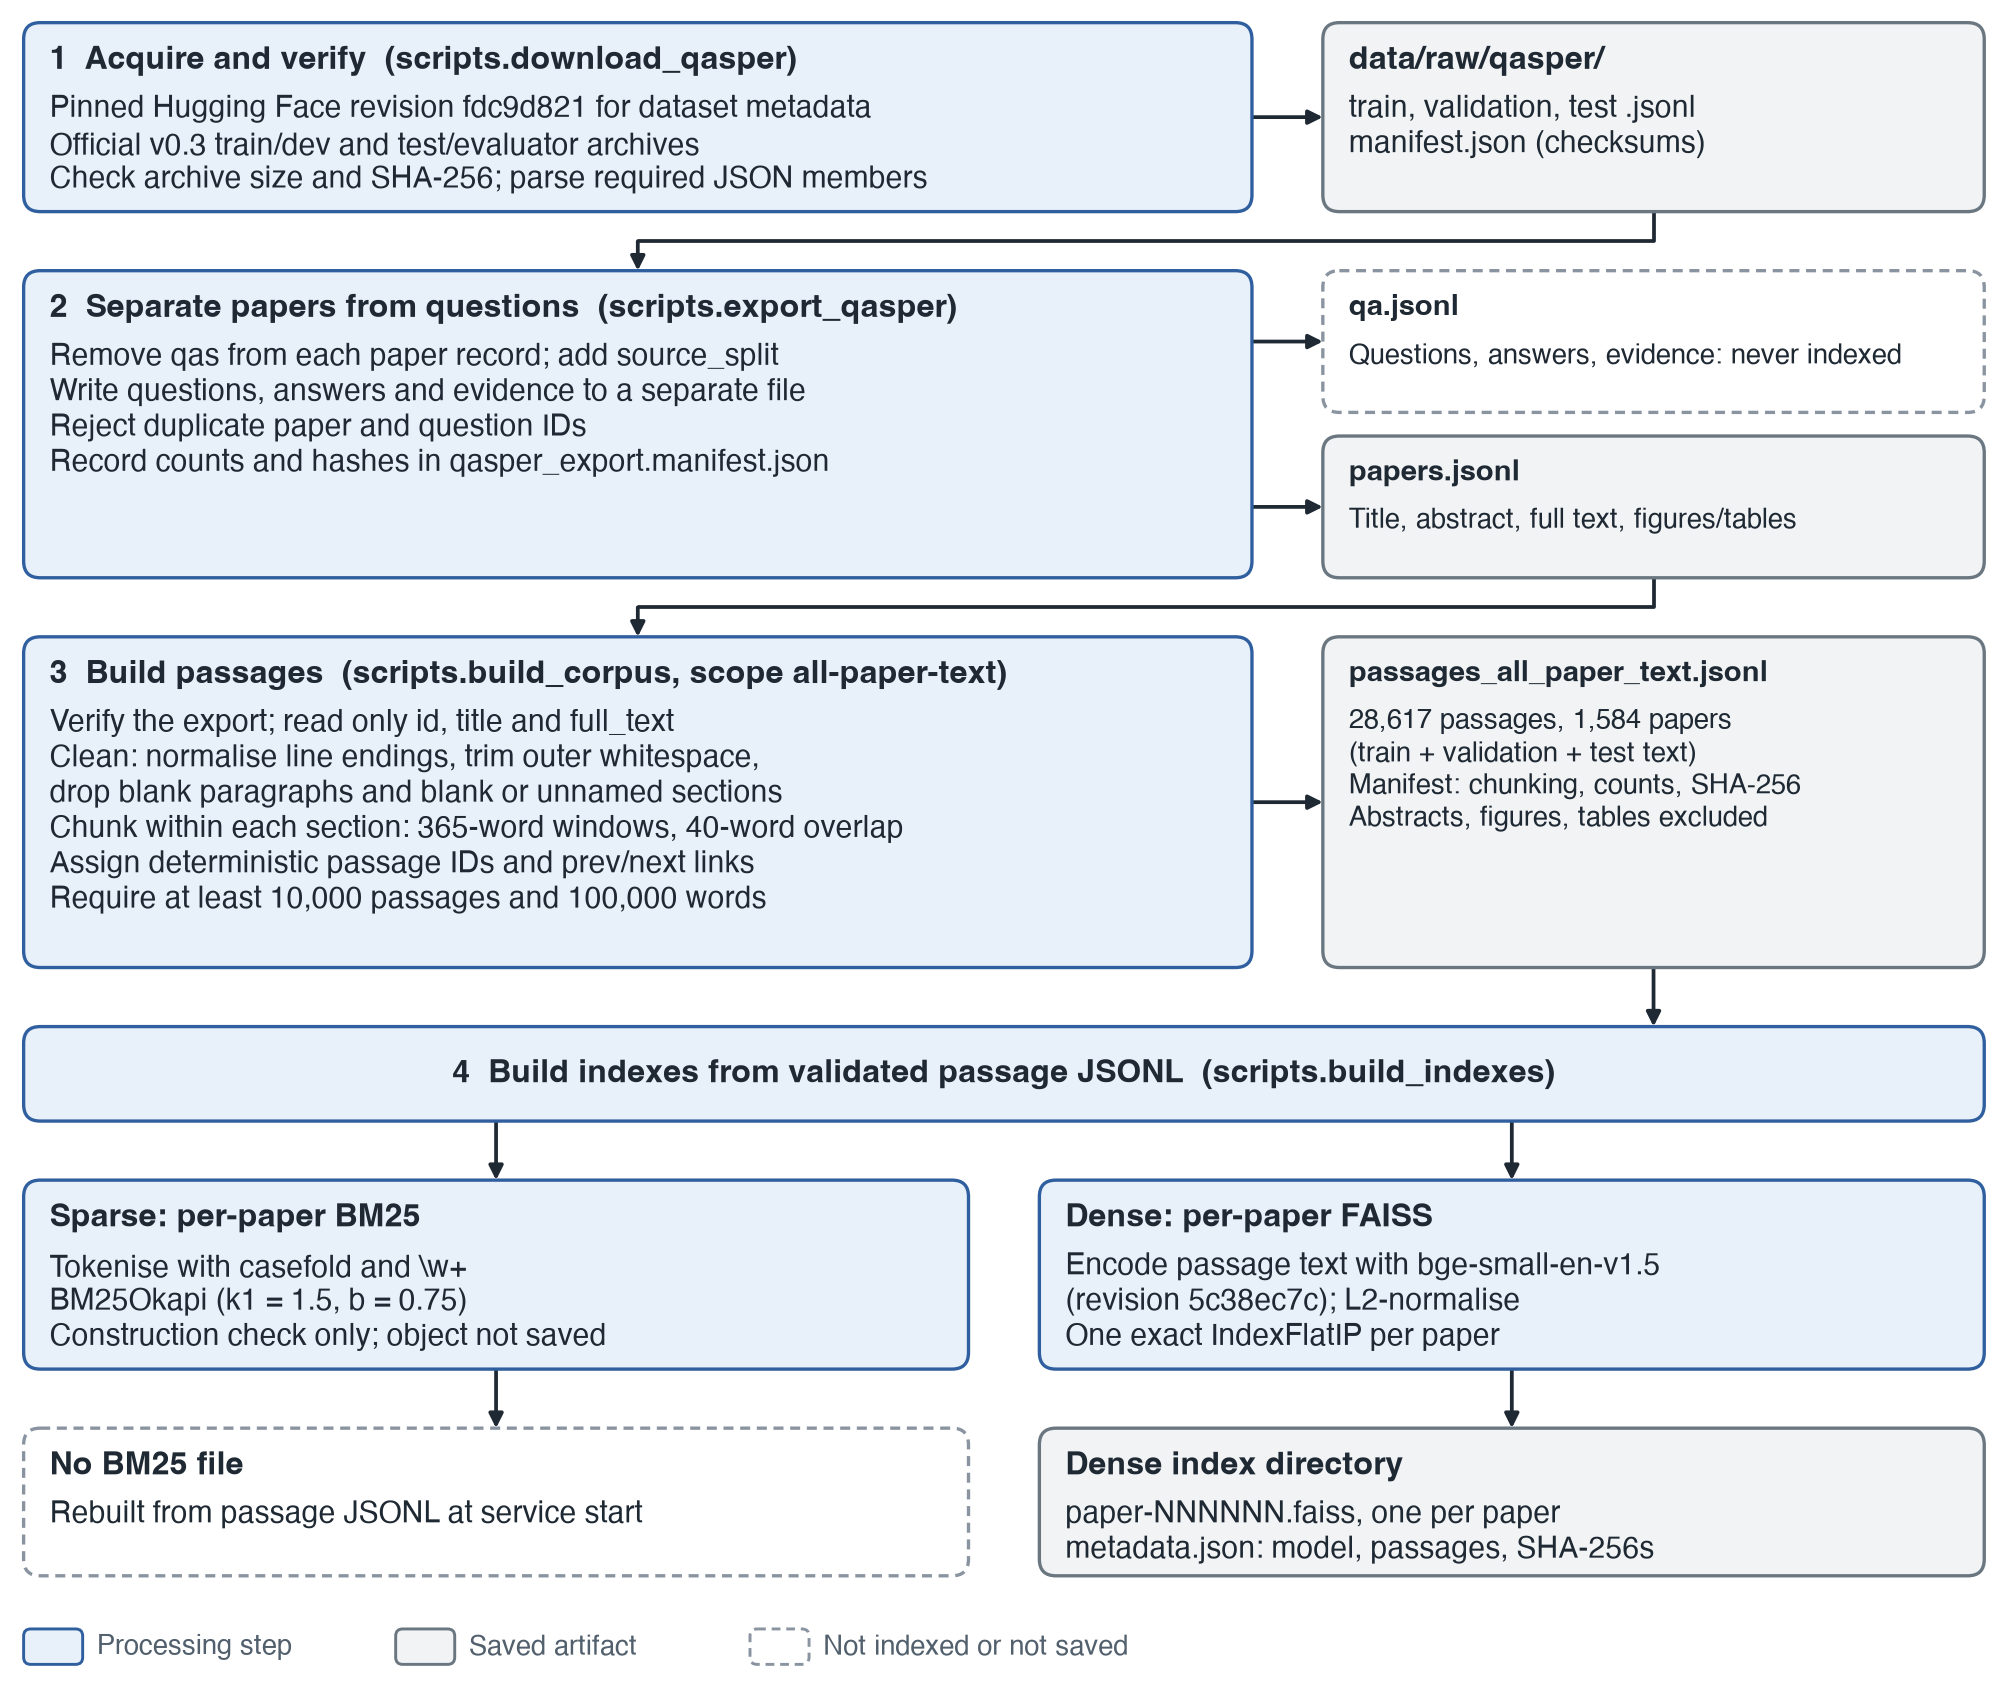
\includegraphics[width=\linewidth,height=0.78\textheight,keepaspectratio]{images/offline-corpus-index.png}
\caption{Offline corpus preparation and index construction. BM25 is reconstructed from passage JSONL when the service starts; dense indexes and their metadata are saved. Abstracts and figure/table text are excluded from the indexed passages.}\label{fig:offline}
\end{figure}


\subsection{Application and scope (Q1.2)}
PaperRAG supports researchers investigating NLP methods and findings through evidence-grounded question answering. It aims to reduce the effort of locating evidence scattered across papers and sections and tracing claims to their sources.

Users enter a natural-language question and choose either a specific paper or the full collection. Selected-paper search supports detailed questions about a paper's methods, datasets, experiments and results. Collection-wide search supports topic exploration by retrieving relevant passages across papers. The system generates an answer with inspectable passage citations, or an explicit refusal when the available evidence is insufficient. Users can open the cited passages to examine the support for individual claims.

Example inputs include:
\begin{itemize}
\item[$\bullet$] \textbf{Selected paper:} ``Which datasets are used to evaluate the proposed method?''
\item[$\bullet$] \textbf{Selected paper:} ``How does the proposed approach differ from the baselines?''
\item[$\bullet$] \textbf{Full collection:} ``What approaches are used for machine translation when parallel training data is limited?''
\item[$\bullet$] \textbf{Full collection:} ``How do entity-linking models use surrounding context to resolve ambiguous names?''
\end{itemize}

The intended benefit is to reduce the effort required to locate and inspect evidence during research. Formal evaluation uses selected-paper questions; collection-wide search is demonstrated separately in Q2.2.


\subsection{Knowledge base size (Q1.3)}
The corpus combines paper text from QASPER's training, validation and test splits. \hyperref[tab:corpus]{Table~\ref*{tab:corpus}} summarizes its size after cleaning and chunking.

\begin{table}[htbp]\centering
\caption{Corpus size for the reported 365/40 chunking configuration.}\label{tab:corpus}
\begin{tabularx}{\linewidth}{>{\hsize=1.4\hsize\linewidth=\hsize}Y>{\hsize=.6\hsize\linewidth=\hsize}Y}\toprule
Measure & Count\\\midrule
Source documents (papers) & 1,585\\
Documents with indexed chunks & 1,584\\
Indexed chunks (passages) & 28,617\\
Source-text words, excluding chunk overlap & 5,659,921\\
Words across chunks, including overlap & 5,930,961\\
Unique word types across chunks & 210,909\\\bottomrule
\end{tabularx}
\end{table}

Words are counted as whitespace-delimited units. Unique types are counted after case folding, with punctuation retained. The chunk-word total is higher because overlapping text is counted in each chunk where it appears. One source paper produces no usable chunks and is therefore absent from the index. The 28,617 chunks and 5,659,921 source-text words exceed the assignment's 10,000-passage and 100,000-word minimums.

\section{System and interface (Q2)}
\subsection{User interface (Q2.1)}


\textbf{Implementation.} We built a web interface using Streamlit, connected to the retrieval and generation pipeline through a FastAPI service. It provides a single place to ask questions and inspect the evidence supporting an answer.

\textbf{Querying.} Users select a specific paper or search across the full collection, enter a natural-language question and submit it. They can also choose an example question to get started. \hyperref[fig:ui-entry]{Figure~\ref*{fig:ui-entry}} shows the input screen with a question entered and the full collection selected.

\textbf{Inspecting results.} The interface displays the generated answer with passage citations and expandable source details. Users can inspect the cited text, evidence status and validation warnings; retrieval history provides further detail when needed. Keeping supporting information expandable makes the main answer easy to read while allowing users to investigate its evidence. \hyperref[fig:ui]{Figure~\ref*{fig:ui}} shows a returned answer and its sources.

\textbf{Interaction scope.} When the system returns a refusal, the interface presents it as an outcome rather than a technical error. Each submitted question is processed independently; displayed session history does not provide conversational memory.

\begin{figure}[htbp]\centering
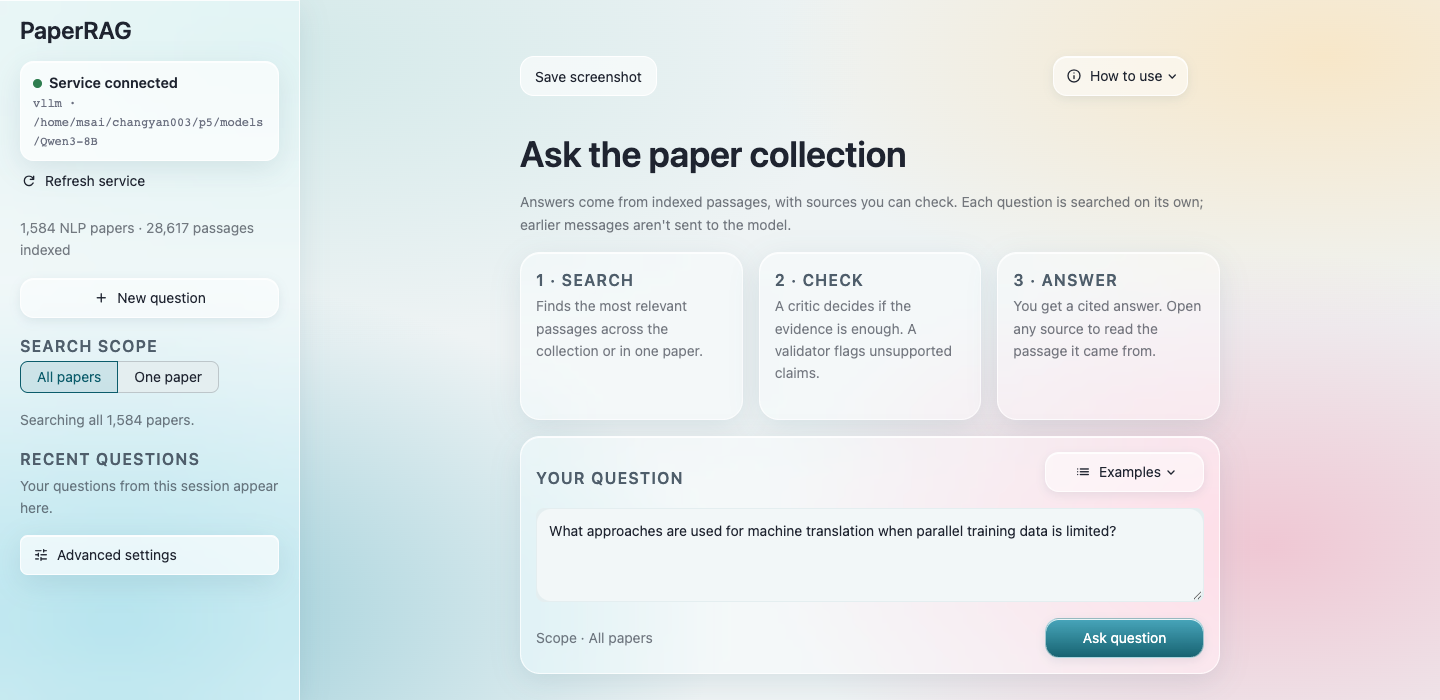
\includegraphics[width=0.97\linewidth]{figures/ui-query-entry.png}
\caption{The interface before submission, with query 3 of \hyperref[tab:queries]{Table~\ref*{tab:queries}} entered and all papers in scope. \hyperref[fig:ui]{Figure~\ref*{fig:ui}} shows the resulting answer.}\label{fig:ui-entry}
\end{figure}

\begin{figure}[htbp]\centering
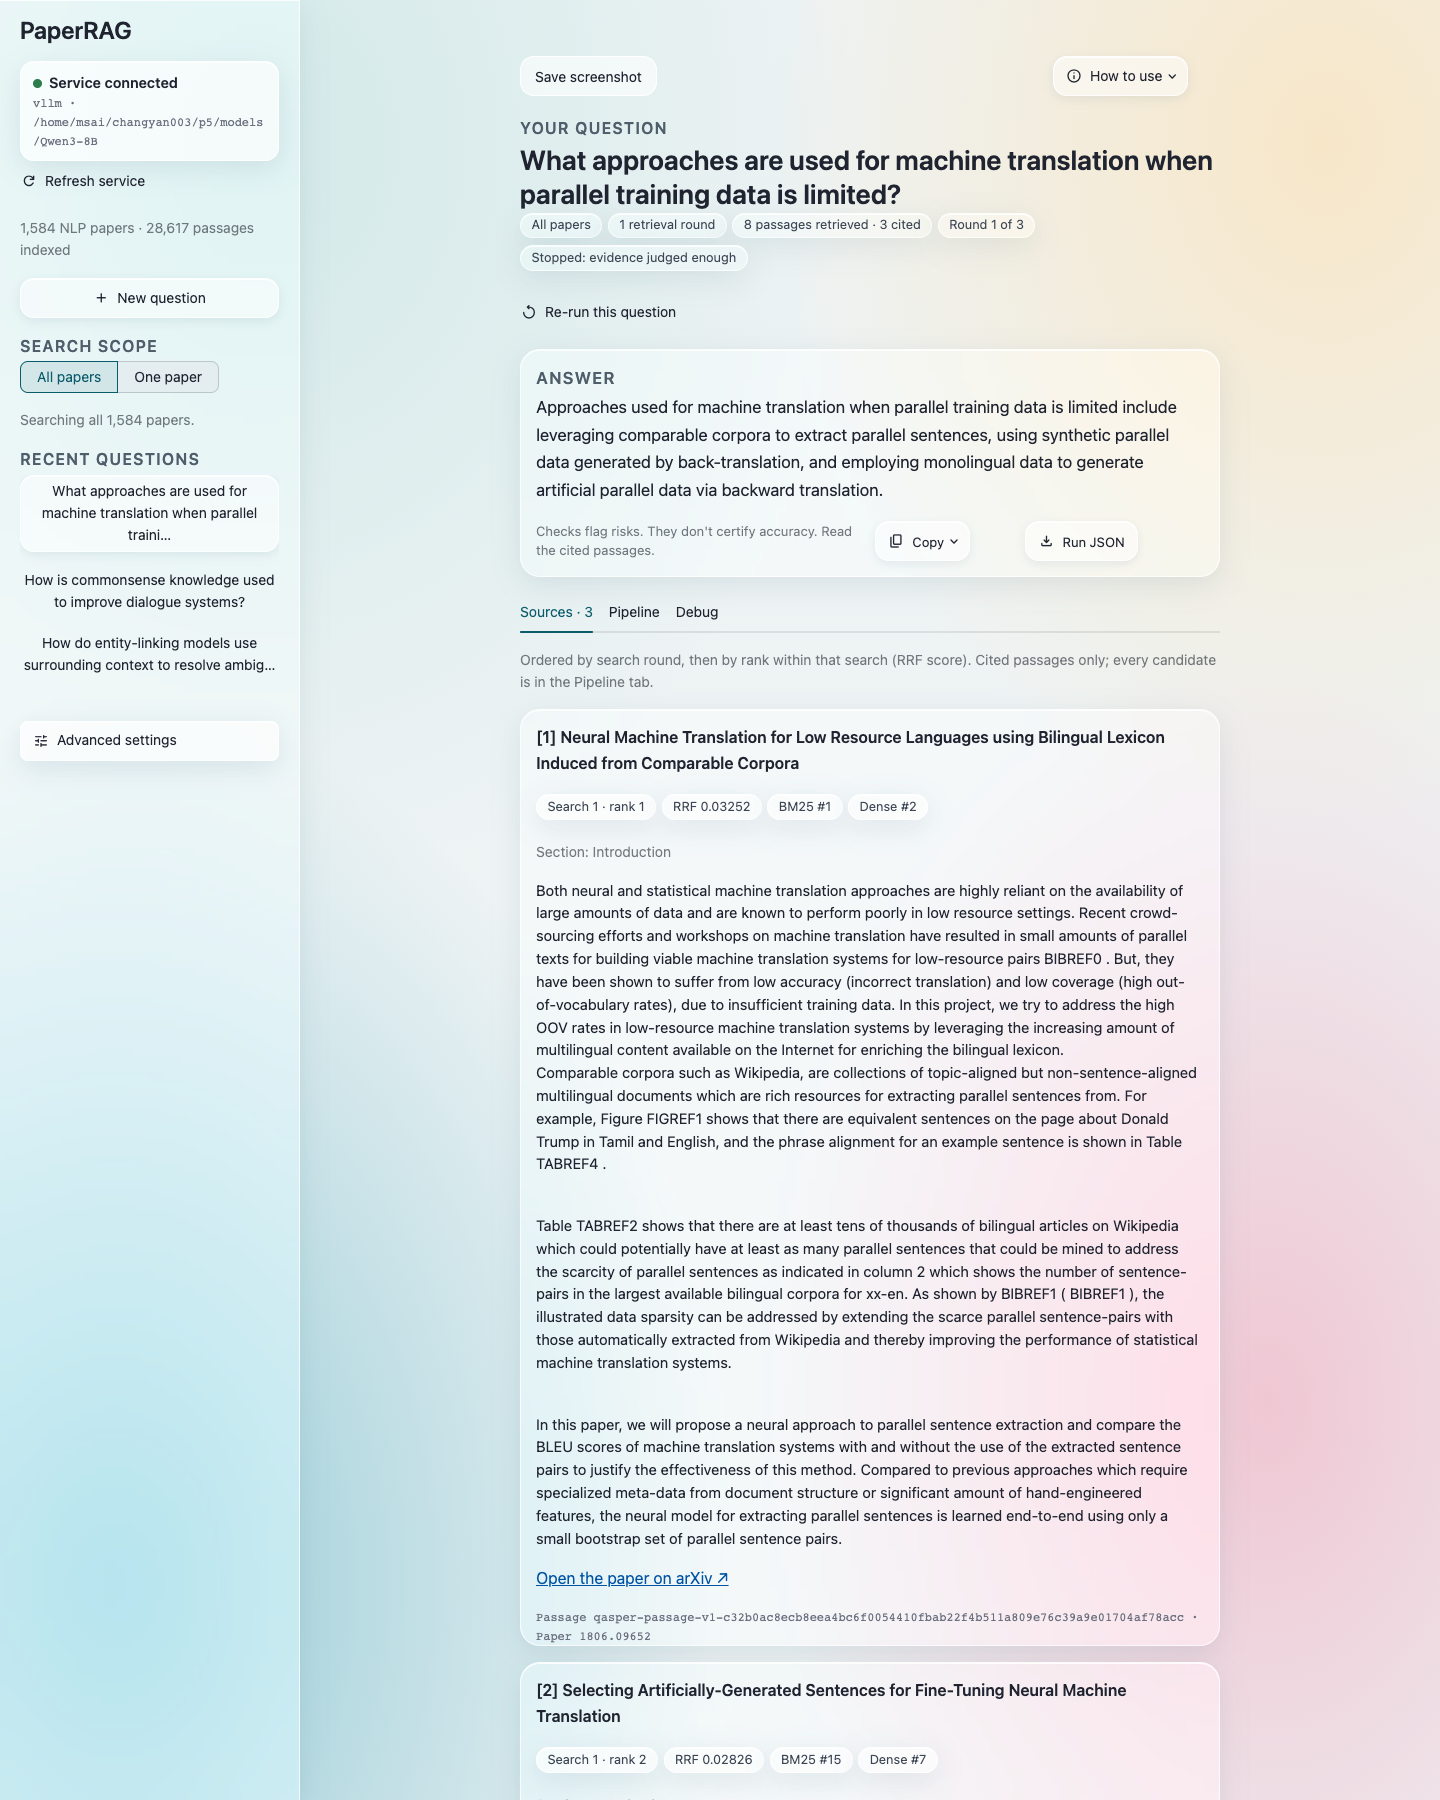
\includegraphics[width=0.97\linewidth,height=0.52\textheight,keepaspectratio]{figures/ui-answer.png}
\caption{The interface answering query 3 of \hyperref[tab:queries]{Table~\ref*{tab:queries}} in a browser against the live GPU service, with all papers in scope. The answer raised no validator warnings, and each source card shows its passage, rank and RRF score. \hyperref[fig:five-queries]{Figure~\ref*{fig:five-queries}} shows how flagged sentences appear.}\label{fig:ui}
\end{figure}

\subsection{Five measured queries (Q2.2)}\label{sec:five-queries}
\par\smallskip
\noindent\begin{minipage}{\linewidth}
\captionsetup{type=table}\small\centering
\caption{The five demonstration queries, run with all papers in scope.}\label{tab:queries}
\begin{tabularx}{\linewidth}{@{}>{\raggedright\arraybackslash}p{5mm}Y@{}}\toprule
\# & Question\\\midrule
1 & How do entity-linking models use surrounding context to resolve ambiguous names?\\
2 & How is commonsense knowledge used to improve dialogue systems?\\
3 & What approaches are used for machine translation when parallel training data is limited?\\
4 & What methods have researchers used to induce context-free grammars (CFGs)? Cite the papers supporting your answer.\\
5 & What methods are used for low-resource language identification?\\\bottomrule\end{tabularx}
\end{minipage}\par\medskip
\begin{table}[htbp]\small\centering
\caption{Summaries of generated outputs, not verified factual answers. Warning counts are validator diagnostics.}\label{tab:five-results}
\begin{tabularx}{\linewidth}{rYrrrr}\toprule
\# & Output summary & Rounds & Cites & Warnings & Seconds\\\midrule
1 & Yes; cross-language vector mapping, checked against Google Translate & 1 & 4 & 2 & 174.2\\
2 & Average classification accuracy & 3 & 1 & 2 & 98.7\\
3 & F1: 88\% on OntoNotes, 53\% on Wiki(gold) & 1 & 1 & 0 & 159.5\\
4 & BiLSTM with max pooling & 1 & 1 & 1 & 104.6\\
5 & Refused: insufficient evidence & 1 & 0 & 0 & 76.3\\\bottomrule\end{tabularx}\end{table}

\textbf{Run setup.} We submitted the five queries in \hyperref[tab:queries]{Table~\ref*{tab:queries}} through the Streamlit interface, with the full collection selected. Requests ran sequentially against the school GPU service using Qwen3-8B through vLLM and top-eight RRF retrieval without reranking. The service was already running; no dedicated warm-up query was used.

\textbf{Results.} \hyperref[tab:five-results]{Table~\ref*{tab:five-results}} summarizes the returned answers, citation counts, validation warnings and latency. \hyperref[fig:five-queries]{Figure~\ref*{fig:five-queries}} shows the corresponding interface outputs. The summaries describe generated responses; warning counts are validator diagnostics.

\textbf{Query speed.} Latency was measured as the client-observed answer HTTP response time, including retrieval, critic processing and answer generation, but excluding subsequent citation lookup and interface rendering. Mean latency was 19.9 seconds, with a median of 19.3 seconds and a range of 15.1--26.3 seconds. Query 5 took longest and required three retrieval rounds; the others required one. Each query was measured once, so these figures describe the demonstration rather than repeated-run performance.

\begin{figure}[htbp]\centering
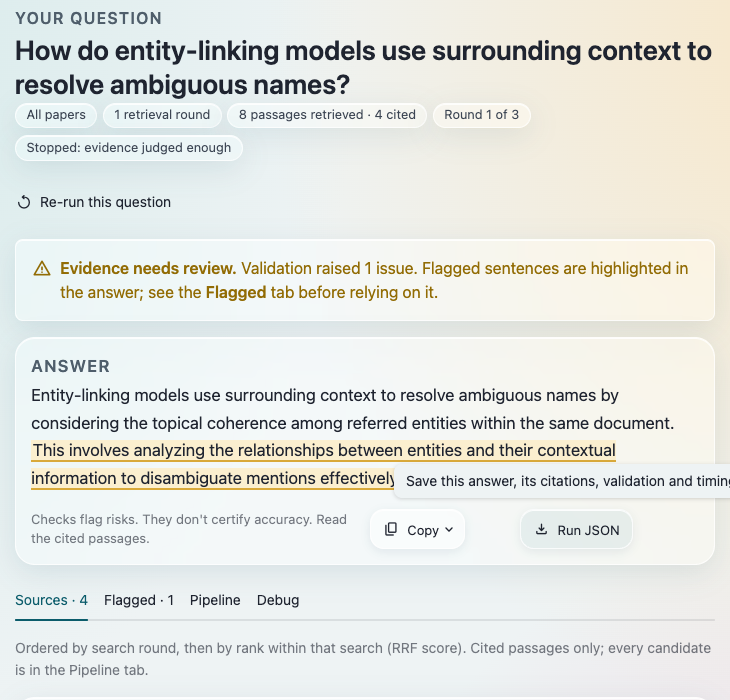
\includegraphics[width=0.48\linewidth]{figures/query-1.png}\hfill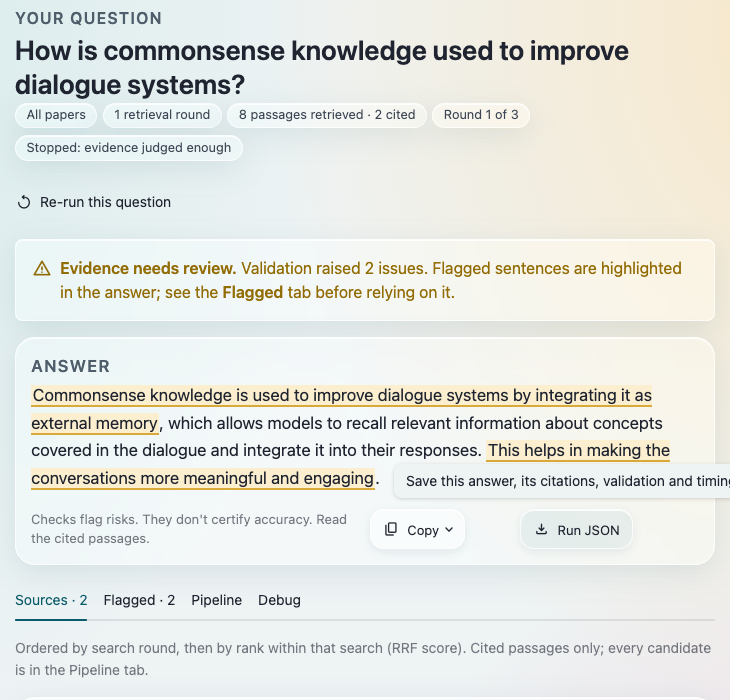
\includegraphics[width=0.48\linewidth]{figures/query-2.png}\\[2mm]
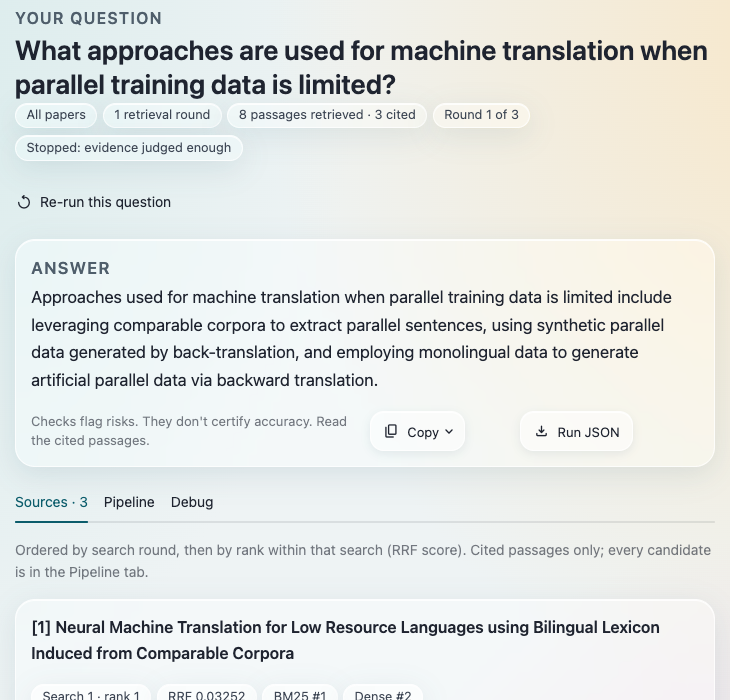
\includegraphics[width=0.48\linewidth]{figures/query-3.png}\hfill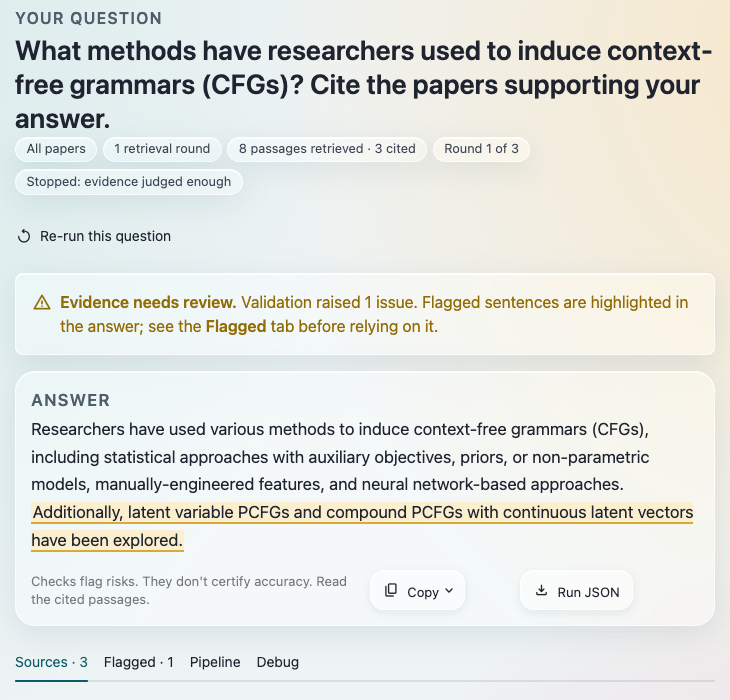
\includegraphics[width=0.48\linewidth]{figures/query-4.png}\\[2mm]
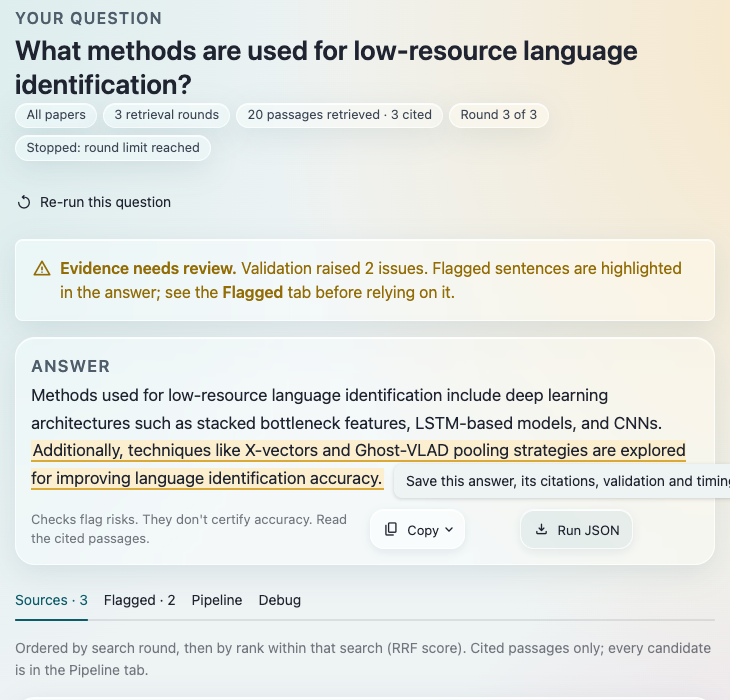
\includegraphics[width=0.48\linewidth]{figures/query-5.png}
\caption{Answers to queries 1--5 as shown by the interface, left to right and top to bottom. Screenshots are cropped to the answer column.}\label{fig:five-queries}
\end{figure}

\textbf{Result observations.} All five queries returned answers, and all 15 citations resolved to passage text. The AI-assisted inspection of cited passages found support for Query 3's listed approaches, while the other outputs contained omissions, unsupported claims or citation mismatches. Query 2's cited passages did not support its dialogue-related answer. Query 4 included a citation mismatch for compound PCFGs and did not name the supporting papers in the answer text, although source cards identified them. Query 5 illustrates the role of source inspection: the system retrieved passages ranked as relevant, but some did not directly support the associated claims. These exploratory queries demonstrate the query workflow and citation inspection; quantitative answer-quality evaluation is reported in Q4.

% Hidden from report; assessment retained in review-checks/q2-2.tex.
% \begin{review}{Q2.2: AI-suggested five-star implementation self-check}
\draftreview{P6}{P5, P4}{P6 verifies the five-query records and timing calculations; P5 checks answer support and citation behavior; P4 investigates critic mismatches.}
\aistars{4}\quad\textbf{Provisional AI assessment (7 November 2026, post-review): 4/5 stars.} This is an editorial assessment of the documented evidence, not a course grade or human sign-off. Five all-papers queries have inputs, output summaries, rounds, citation and warning counts, timings and screenshots. The prose checks grounding against cited passages and identifies confident unsupported answers, including critic/generator disagreement. Hardware and timing boundaries are stated. One serial pass without reference answers cannot estimate accuracy or latency variability; the run export does not fix the job identifier or passage budget, and the AI-assisted grounding check still needs P5/P4 confirmation.
\end{review}

